
\section{Additional analysis of calibration convergence}

In the main analysis described above, each of the seven chains of the adaptive Metropolis algorithm was initialised by adding random noise around parameter values obtained from a previous calibration. This approach was used to assist the algorithm to reach the parameter space's high posterior areas within a reasonable number of iterations. The high number of dimensions ($N=18$) made other approaches such as Latin-Hypercube-based initialisation impractical, as chains could take millions of iterations before adequately sampling plausible parameter sets.

In a separate experiment, we ran another adaptive Metropolis algorithm where only ten parameters were varied, but this time initialisation was performed with Latin Hypercube Sampling (LHS) across ten independent chains. The ten parameters were selected based on their expected influence on the main findings and whether they were among the primary estimands of interest (e.g. the face coverings effect parameter). The remaining eight parameters were fixed to the maximum a-posteriori value obtained in the main analysis. The aim of this analysis was to verify that the calibration algorithm could recover similar convergence to that obtained in the main analysis despite starting from highly diverse initial points.

Figures \ref{fig:lhs_experiments_likelihood} and \ref{fig:lhs_experiments_traces} illustrate the progression of the parameters during this experiment. The parameter traces were compared against the posterior distributions obtained from the main analysis (Figure \ref{fig:lhs_experiments_traces}). We found that the chains converged to similar values when considering the LHS-based calibration compared to the original analysis. The posterior ranges obtained with the LHS-based analysis were sometimes slightly narrower compared to the original calibration. This is attributable to the fact that more parameters were fixed throughout calibration in the LHS-based calibration than in the original calibration. Consequently, more constraints were imposed on the varied parameters that were previously found to be correlated with parameters that have been fixed in the LHS-based analysis.

\begin{figure}[ht]
    \resizebox{1\textwidth}{!}{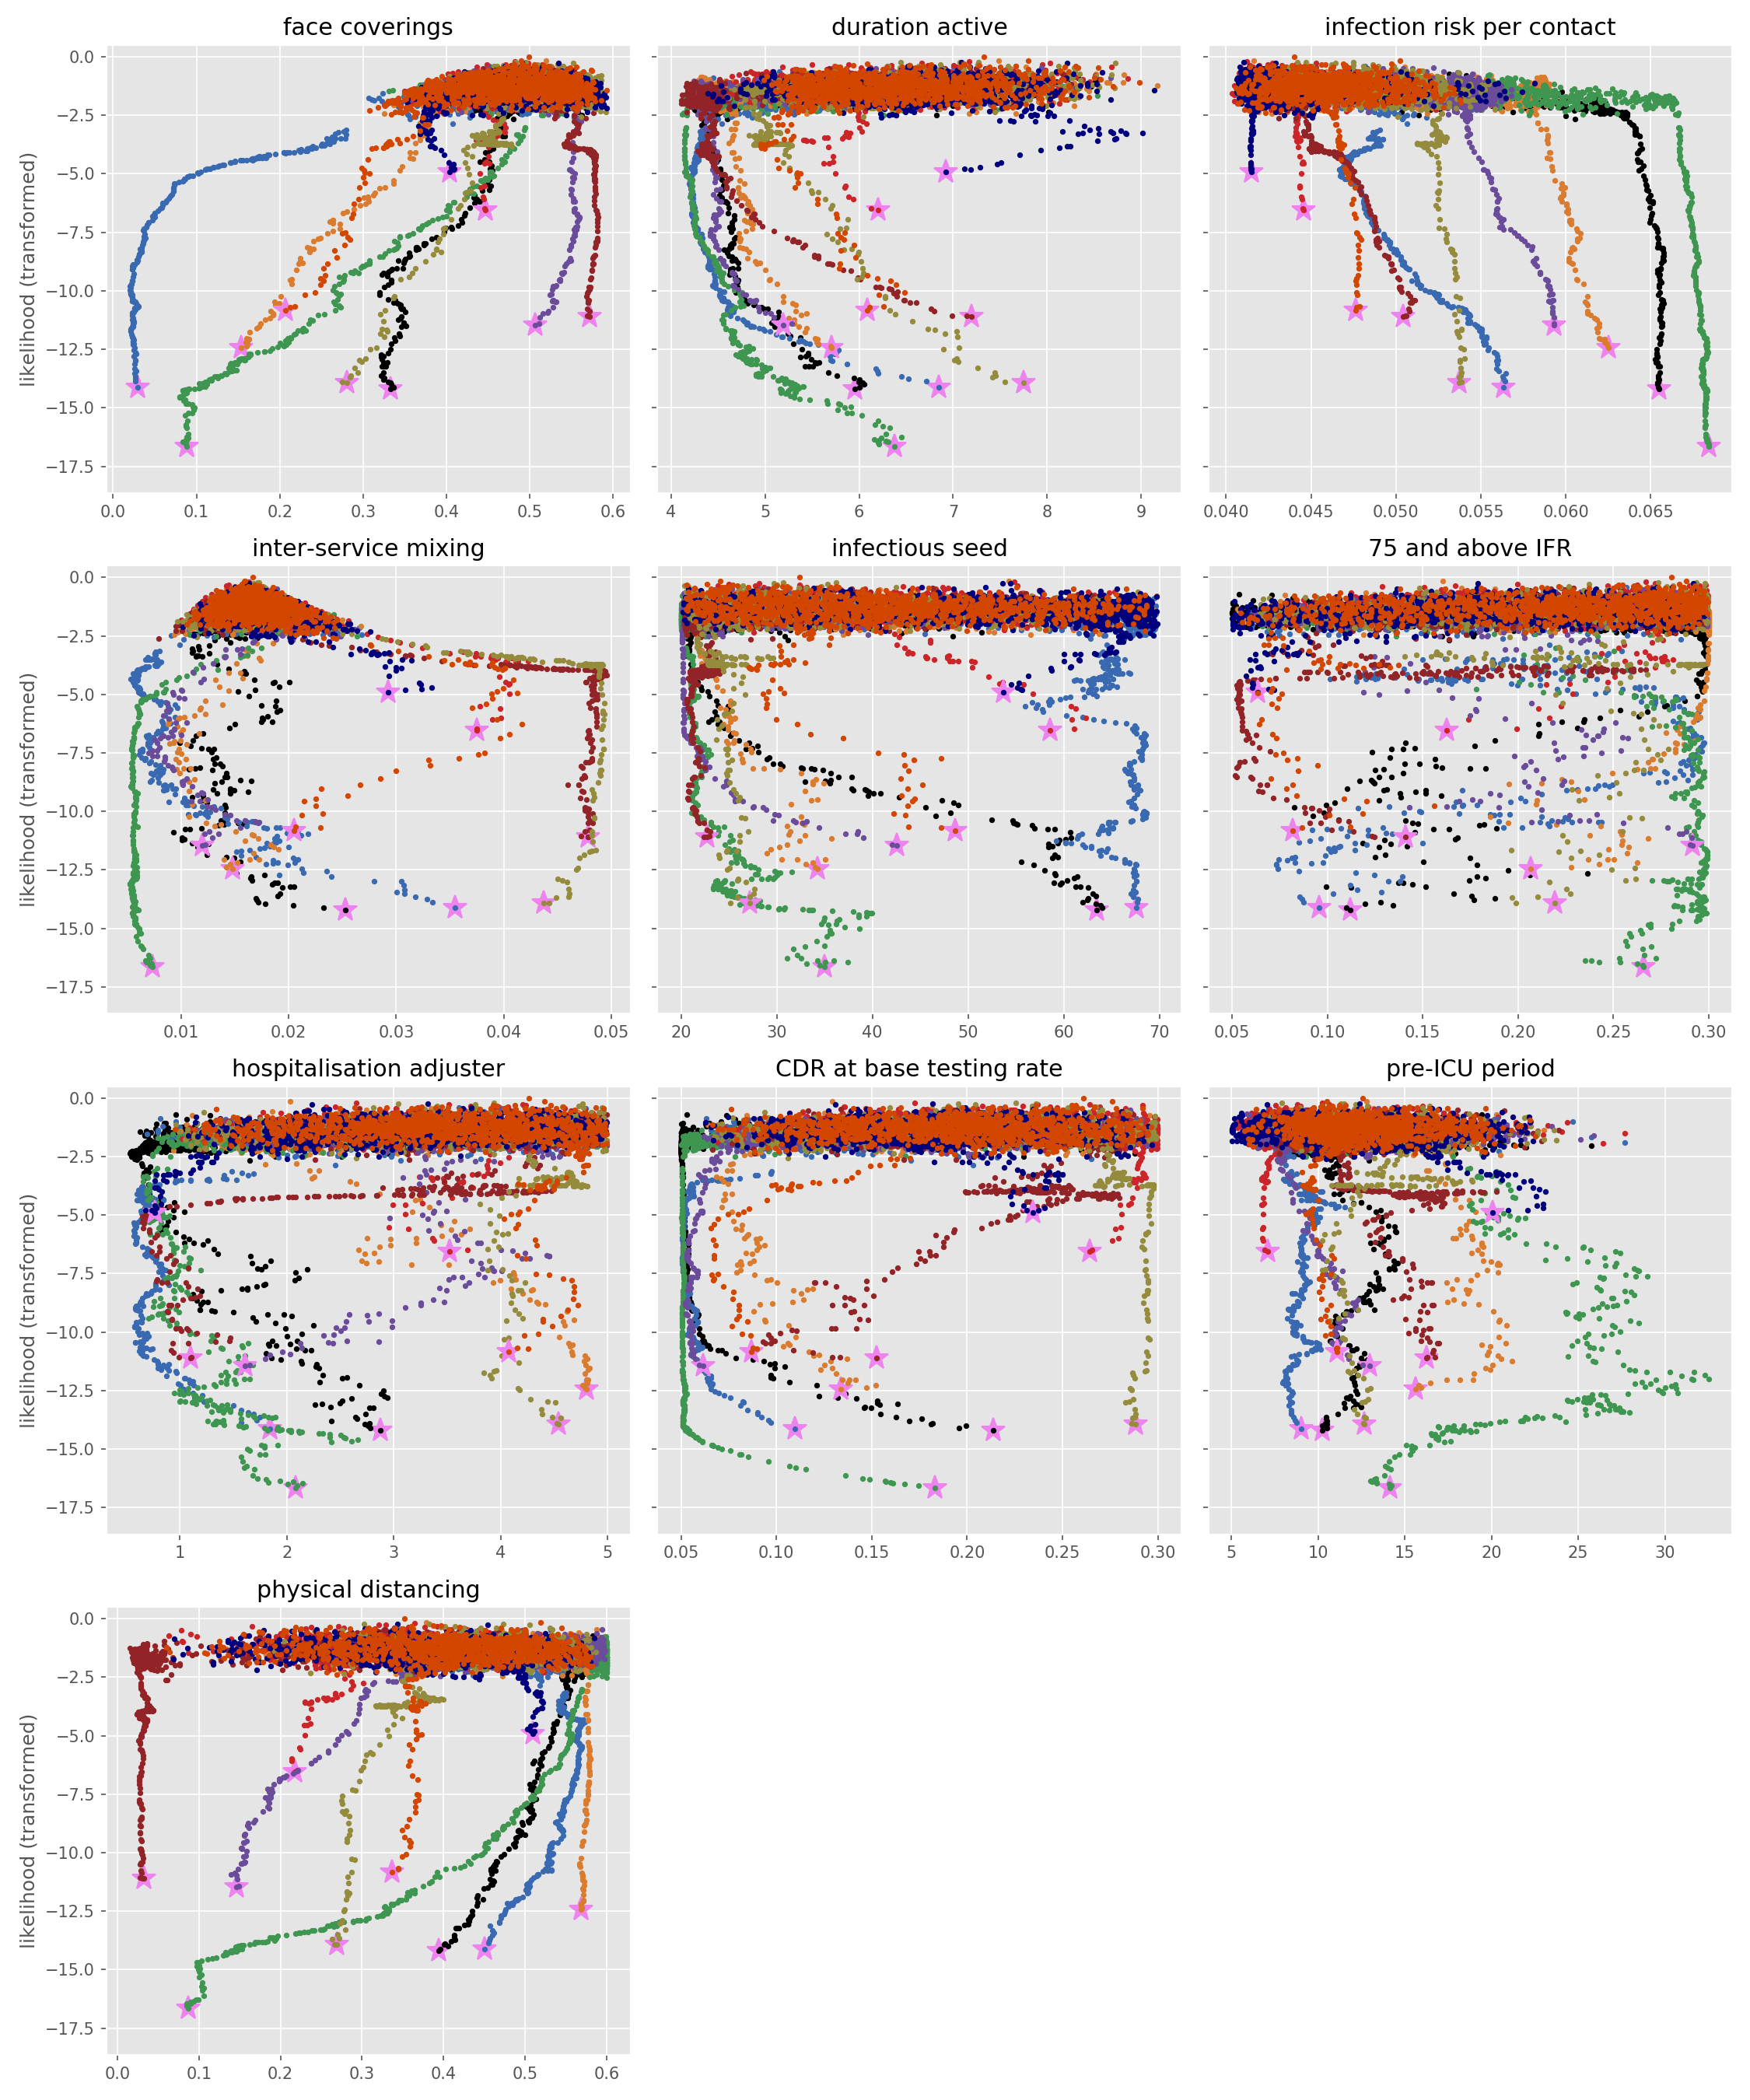
\includegraphics[scale=1]{../covid_19/projects/victoria/lhs_experiments/likelihood_against_params.png}}
    \caption{\textbf{  
	Likelihood against ten key parameters during calibration initialised with Latin Hypercube Sampling.    
    } 
The different colours represent the ten independent adaptive Metropolis chains initialised with Latin Hypercube Sampling. The likelihood values were transformed to increase clarity using $x \rightarrow -log(-log(x) + m + 1)$, where $m$ is the maximum log-likelihood value. The pink stars highlight the starting points.     
    }
    \label{fig:lhs_experiments_likelihood}
\end{figure}


\begin{figure}[ht]
    \resizebox{1\textwidth}{!}{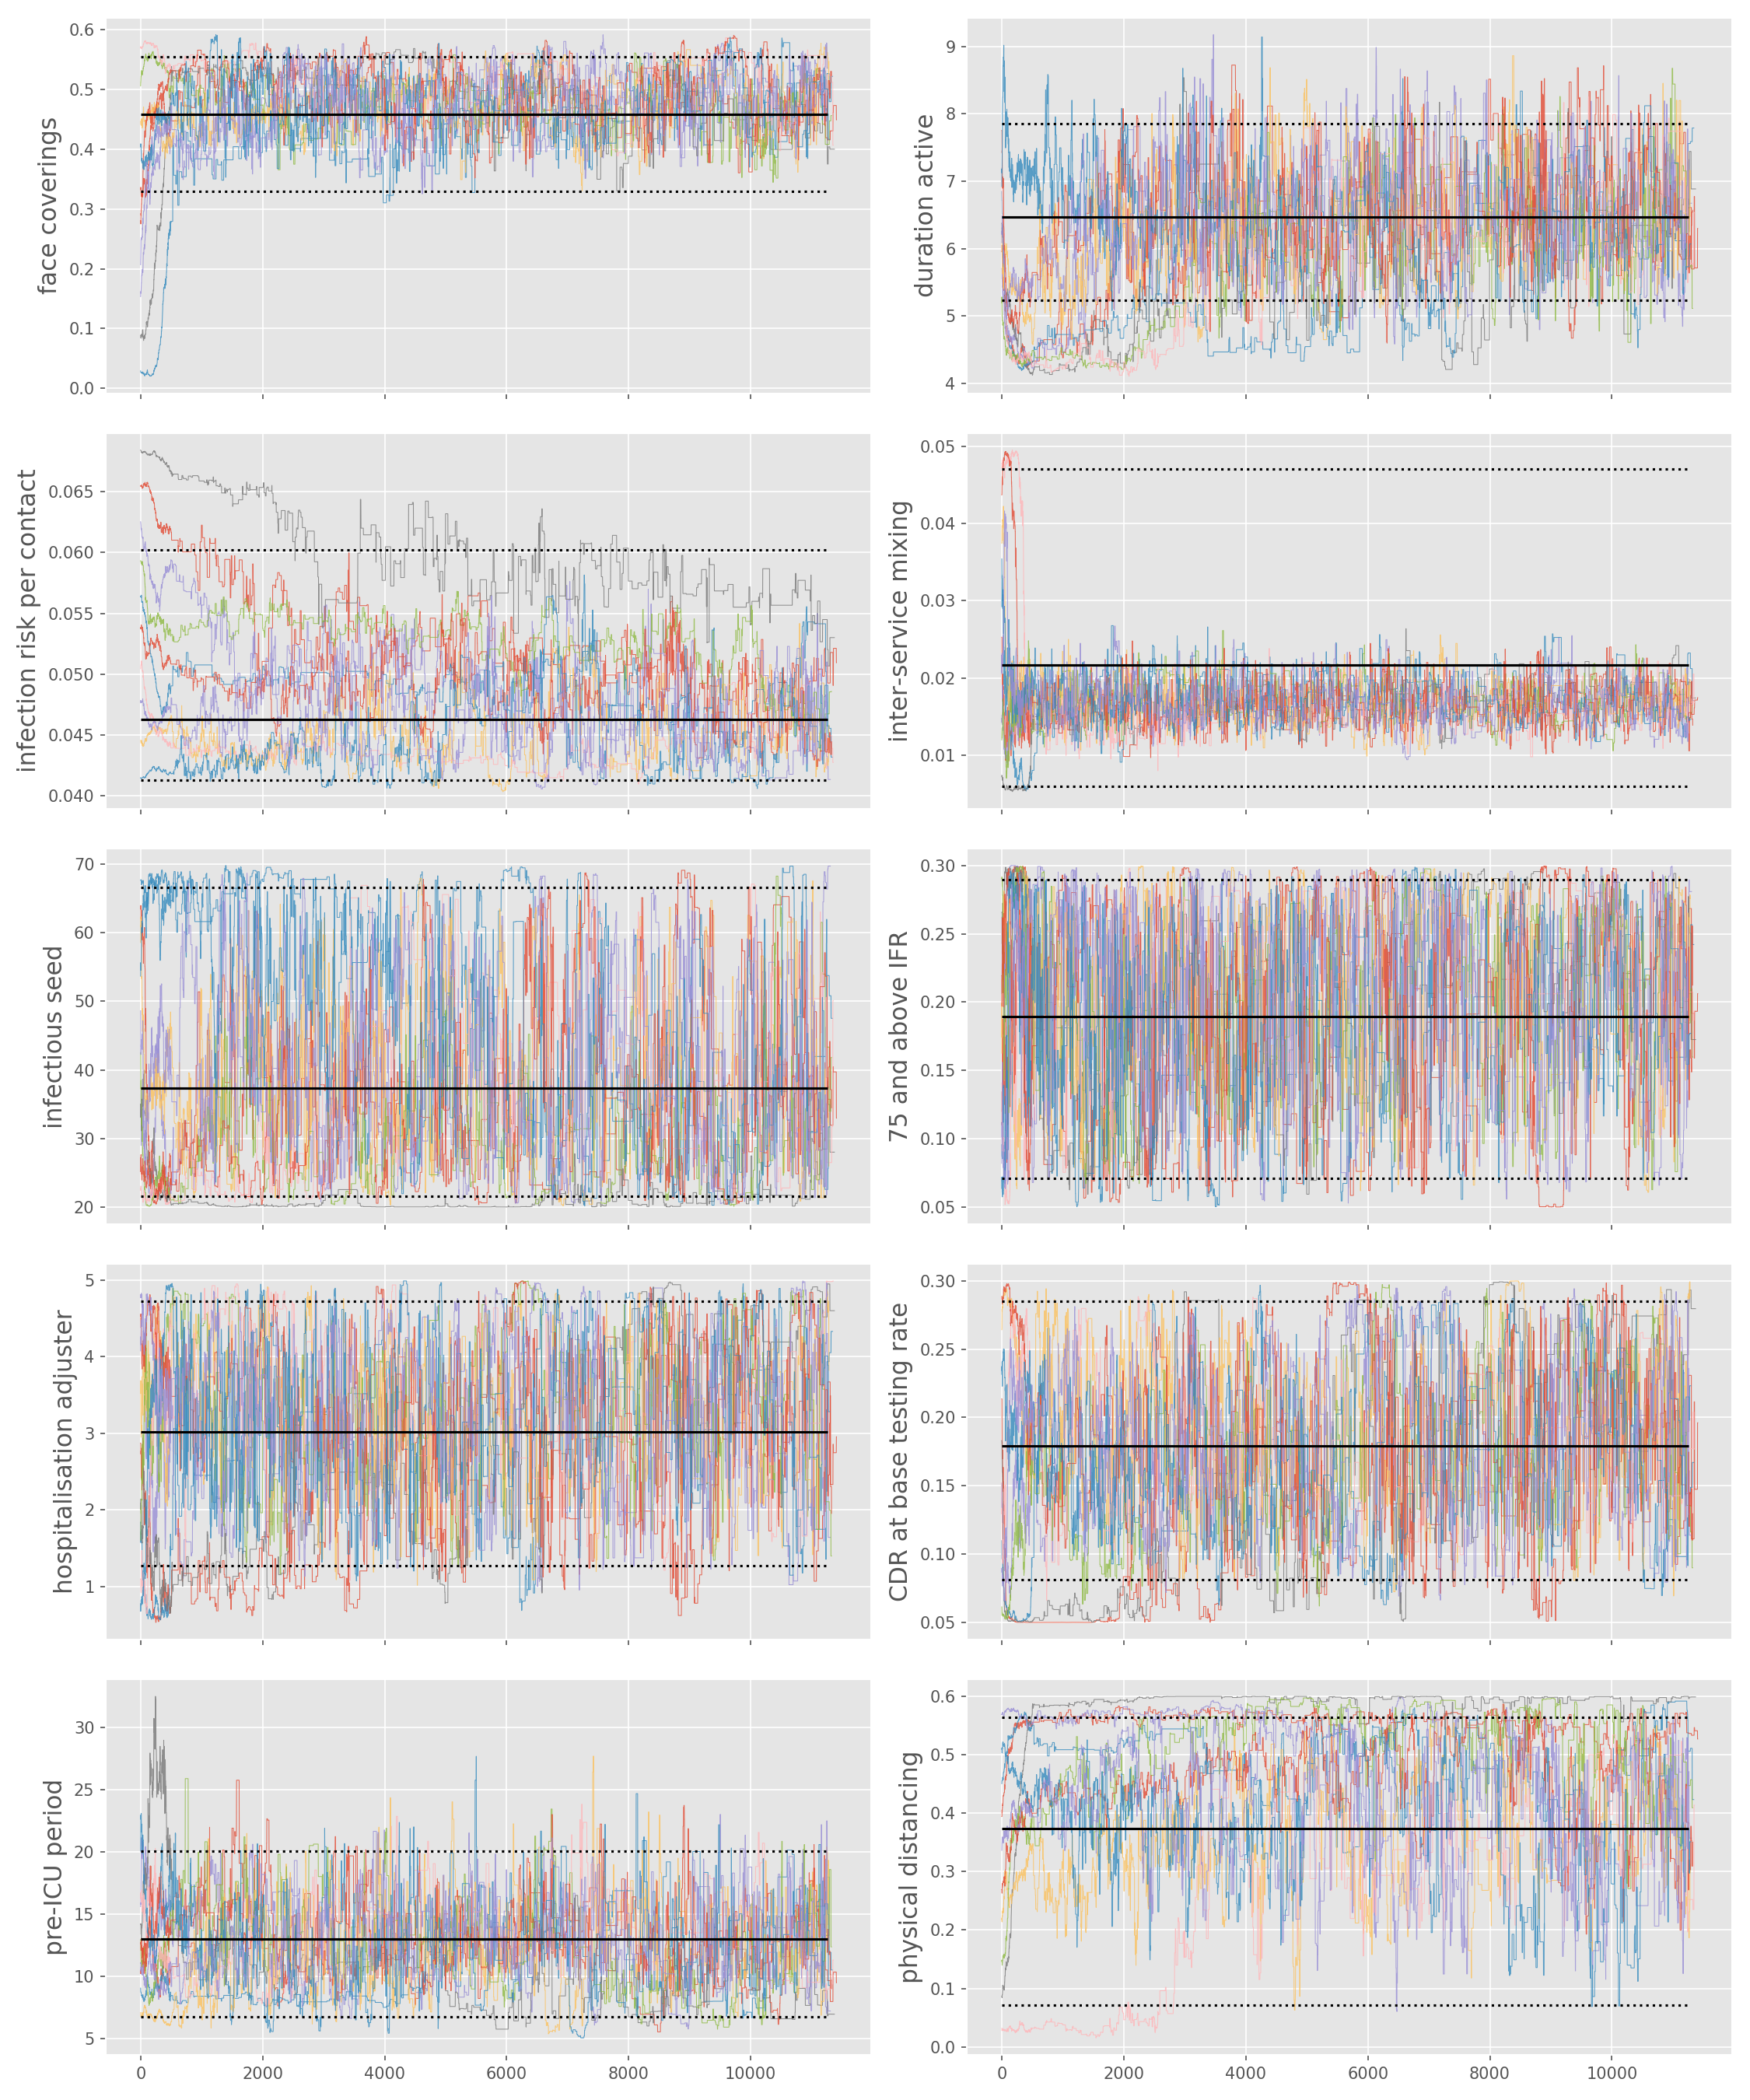
\includegraphics[scale=1]{../covid_19/projects/victoria/lhs_experiments/lhs_start_traces_median.png}}
    \caption{\textbf{Parameter progression traces during calibration initialised with Latin Hypercube Sampling.} The horizontal lines represent the median (solid line) and 95\% credible interval (dotted lines) of the posterior estimates obtained in the main analysis.}
    \label{fig:lhs_experiments_traces}
\end{figure}